% !TEX program = xelatex

\documentclass[12pt,a4paper]{ctexart}
\usepackage{graphicx}
\usepackage{caption}
\usepackage{subcaption}
\usepackage{float}
\usepackage{geometry}
\usepackage{hyperref}
\usepackage{amsmath}
\usepackage{listings}
\usepackage{xcolor}

\geometry{left=2.54cm,right=2.54cm,top=2.54cm,bottom=2.54cm}

\title{计算机图形学 HW2：Image Warping 实验报告}
\author{胡广理 \quad 学号：PB24010500}
\date{\today}

\begin{document}
\maketitle

\section{实验目的}
本实验旨在理解并实现图像变形（Image Warping）算法。深入学习面向对象编程（OOP）思想，将数学映射机制抽象并与具体的图像解耦。具体任务包括：
\begin{itemize}
    \item 结合高斯消元求解线性方程组，实现逆向映射法。
    \item 实现 Inverse Distance-Weighted interpolation (IDW) 算法。
    \item 实现 Radial Basis Functions interpolation (RBF) 算法。
    \item \textbf{选做部分}：使用 ANN (Approximate Nearest Neighbors) 算法实现原图正向映射留下的白缝填补。
    \item \textbf{选做部分}：使用 Dlib 构建轻量级神经网络（MLP）完成图像变形控制点的拟合与预测。
\end{itemize}

\section{算法原理解析}
\subsection{反向映射 (Inverse Mapping)}
正向映射在将图像控制点坐标向目标坐标转换时，极易由于坐标经量化向整数取整的计算方式引起渲染画面产生像素孔洞。因此作业采用了反向映射：遍历目标图像（变形后）上的每个像素坐标，利用映射函数 $f$ 查找其位于源图像上的对应坐标信息（带浮点数），最后采样该位置的颜色，以完美消除基本的无映射空隙。

\subsection{逆距离加权 (IDW)}
通过反距离加权，目标位置由于各个控制点产生的位移权重随着距离控制点的函数呈现负次幂关系：
$$w_i(x) = \frac{1}{\| x - q_i \|^\mu}$$
最终位置将受到多个控制点拉扯位移的加权平均影响。

\subsection{径向基函数 (RBF)}
RBF 使用特定的径向基函数 $\phi(r) = \sqrt{r^2 + d^2}$ 组合一组仿射变换：
$$f(x) = \sum_{i=1}^n \alpha_i \phi(\|x - q_i\|) + A x + b$$
为了求出其中的回归系数 $\alpha, A, b$，在 \verb|RBF_warper.cpp| 中构建了原生的高斯消元法针对选定矩阵进行求解。

\section{核心代码及选做项说明}
\begin{itemize}
    \item \textbf{抽象与多态}：设计了 \verb|Warper| 基类，包含 \verb|init()| 和虚函数 \verb|warp(x, y, out_x, out_y)|，实现解耦。子类 \verb|IDWWarper| 和 \verb|RBFWarper| 重写了该推断逻辑。
    \item \textbf{ANN补缝 (Gap Filling)}：整合了轻量级 \verb|annoy| 库。对因鱼眼（Fisheye）等前向映射遗留的空洞区间像素，在颜色缓存树中查找最近邻域的映射点对其颜色进行补全（即Gap Filling）。
    \item \textbf{Dlib 神经网络}：编写 \verb|Dlib_warper| 和 CMake 预处理宏。构造了两层 \verb|fc<16>| 及 ReLU 激活的全连接层神经网络结构。以已标定控制点为训练集，利用 \verb|dnn_trainer| 在每次变形时进行拟合训练并推理预测全局坐标差。
\end{itemize}

\section{实验结果展示}
实验测试平台使用了 Lenna 图以及黑白棋盘格作为评估基准。在成功执行各项模块代码后得到的运行成果展示如下：

\subsection{常规映射结果 (IDW/RBF)}
结合抽象底层算法实现的局部多控制点平滑控制。
\begin{figure}[H]
    \centering
    \begin{subfigure}{0.45\textwidth}
        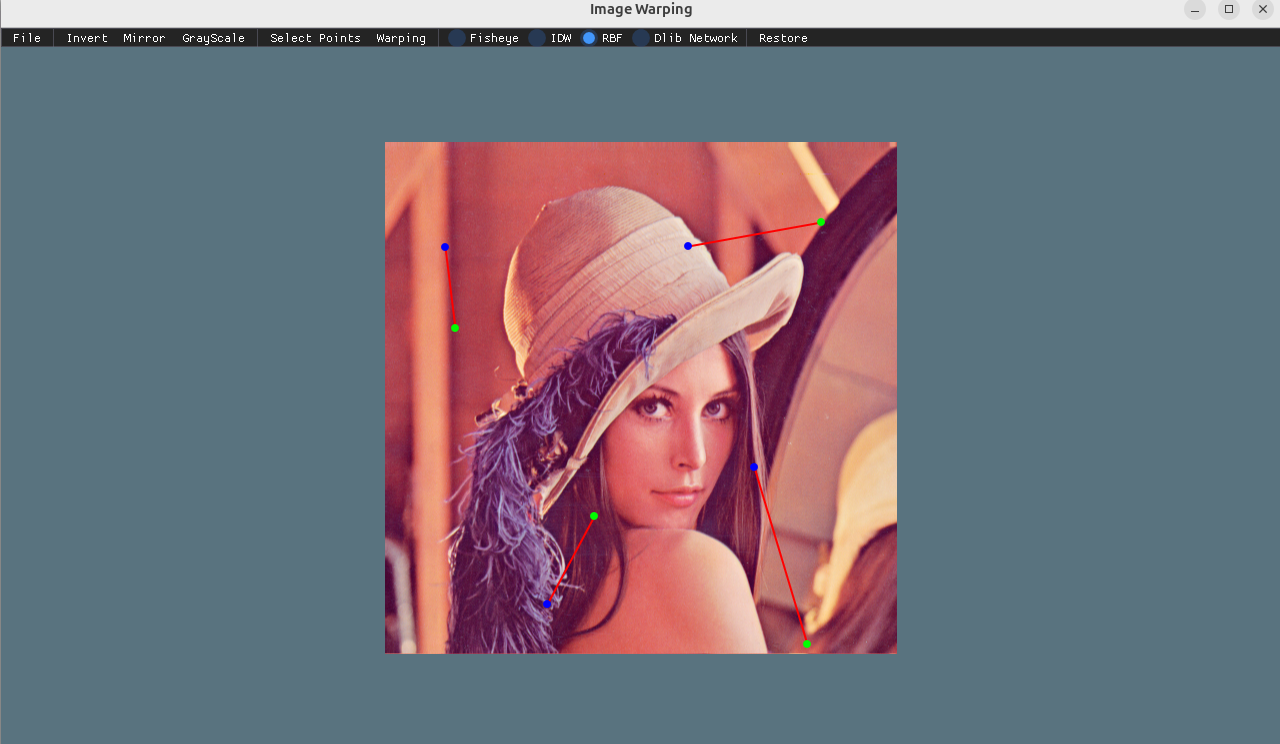
\includegraphics[width=\textwidth]{example_pictures/lenna标点.png}
        \caption{Lenna 加标控制点}
    \end{subfigure}
    \hfill
    \begin{subfigure}{0.45\textwidth}
        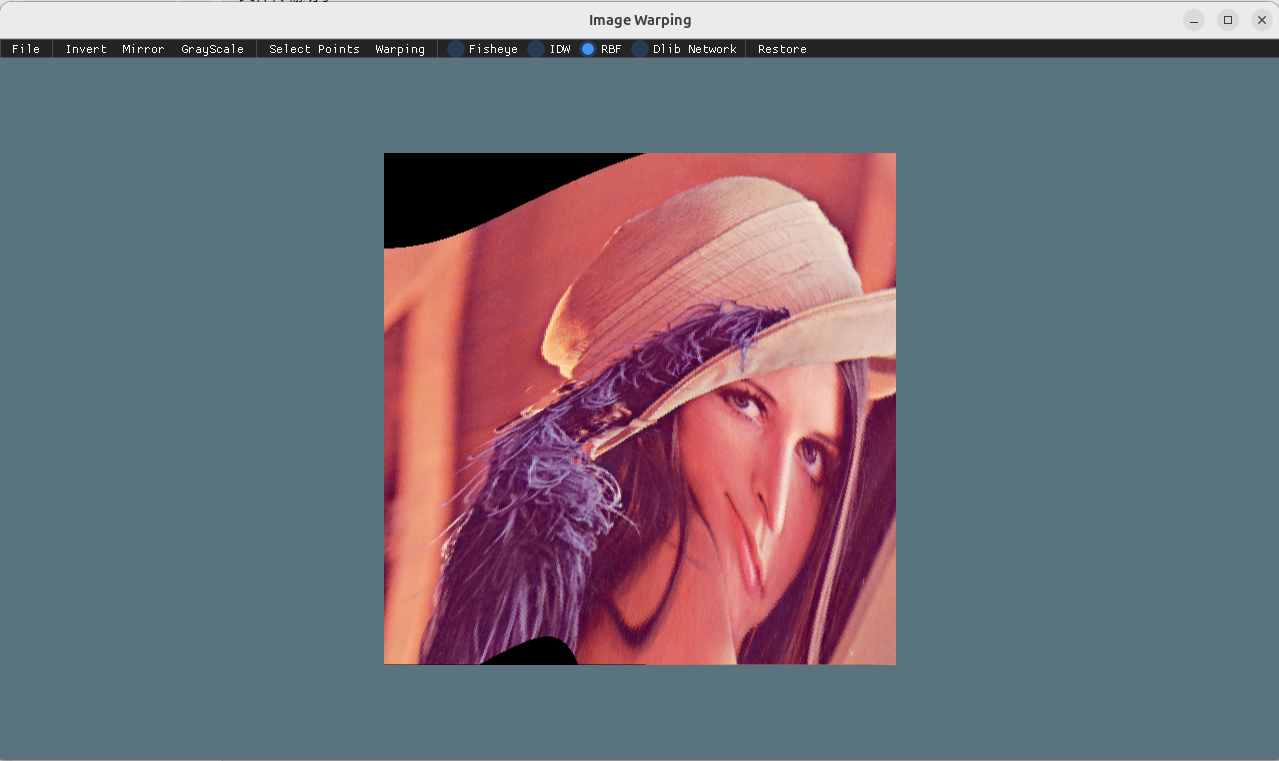
\includegraphics[width=\textwidth]{example_pictures/lenna标点之后转化.png}
        \caption{Lenna Warping 结果}
    \end{subfigure}
    \caption{Lenna图像形变效果}
\end{figure}

\begin{figure}[H]
    \centering
    \begin{subfigure}{0.45\textwidth}
        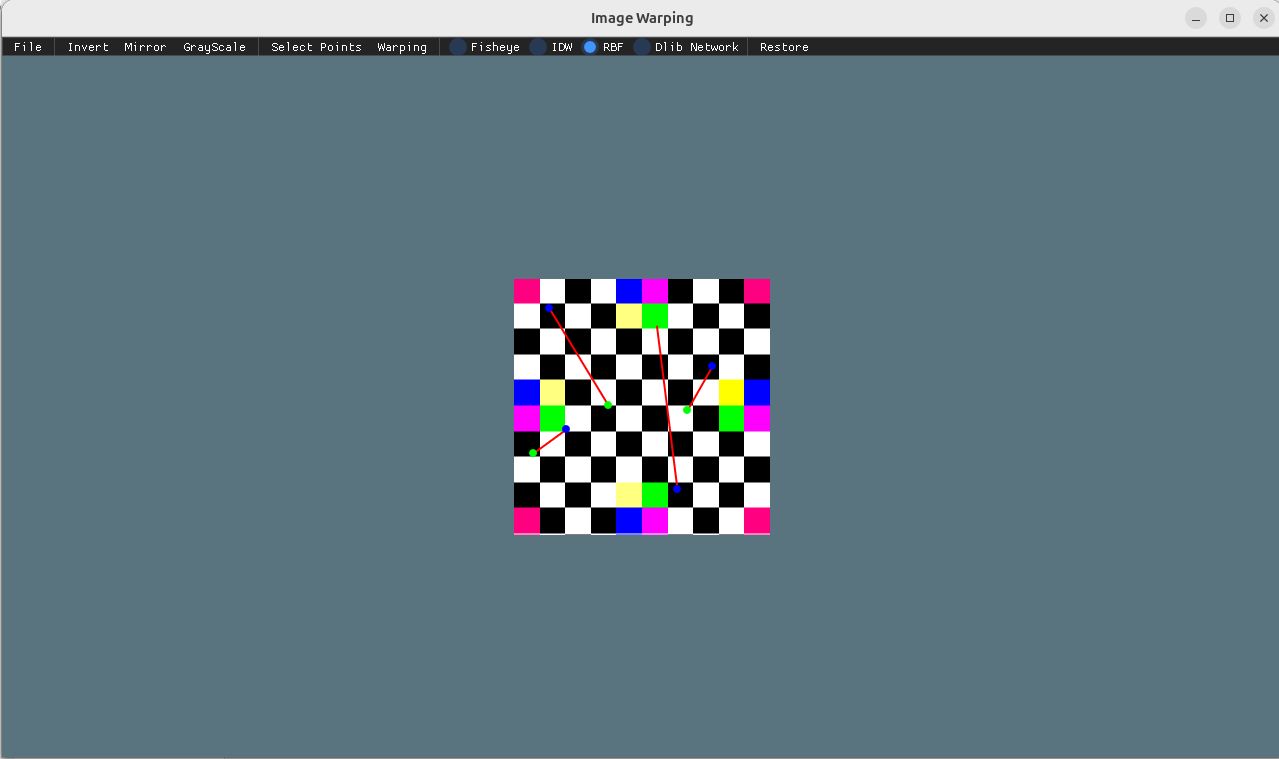
\includegraphics[width=\textwidth]{example_pictures/棋盘格标点.png}
        \caption{棋盘格 加标控制点}
    \end{subfigure}
    \hfill
    \begin{subfigure}{0.45\textwidth}
        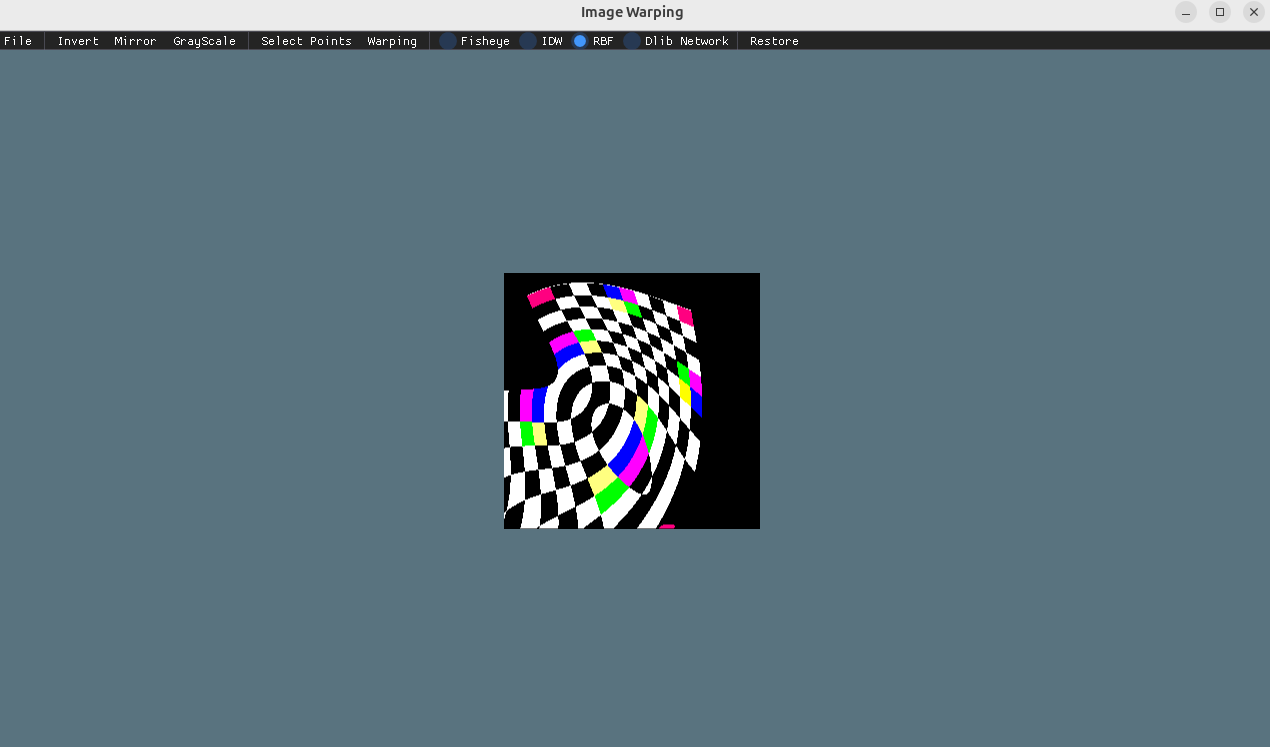
\includegraphics[width=\textwidth]{example_pictures/棋盘格标点之后转化.png}
        \caption{棋盘格 Warping 结果}
    \end{subfigure}
    \caption{棋盘格网格检测形变测试}
\end{figure}

\subsection{鱼眼形变及 ANN 白缝填补效果}
通过调用 Fisheye 等前向投射，并辅以可选任务要求中的 ANN（K-D Tree 近邻查找结构）填补周围缝隙，生成的最终图像没有离散的白洞缝隙，表现平滑。
\begin{figure}[H]
    \centering
    \begin{subfigure}{0.45\textwidth}
        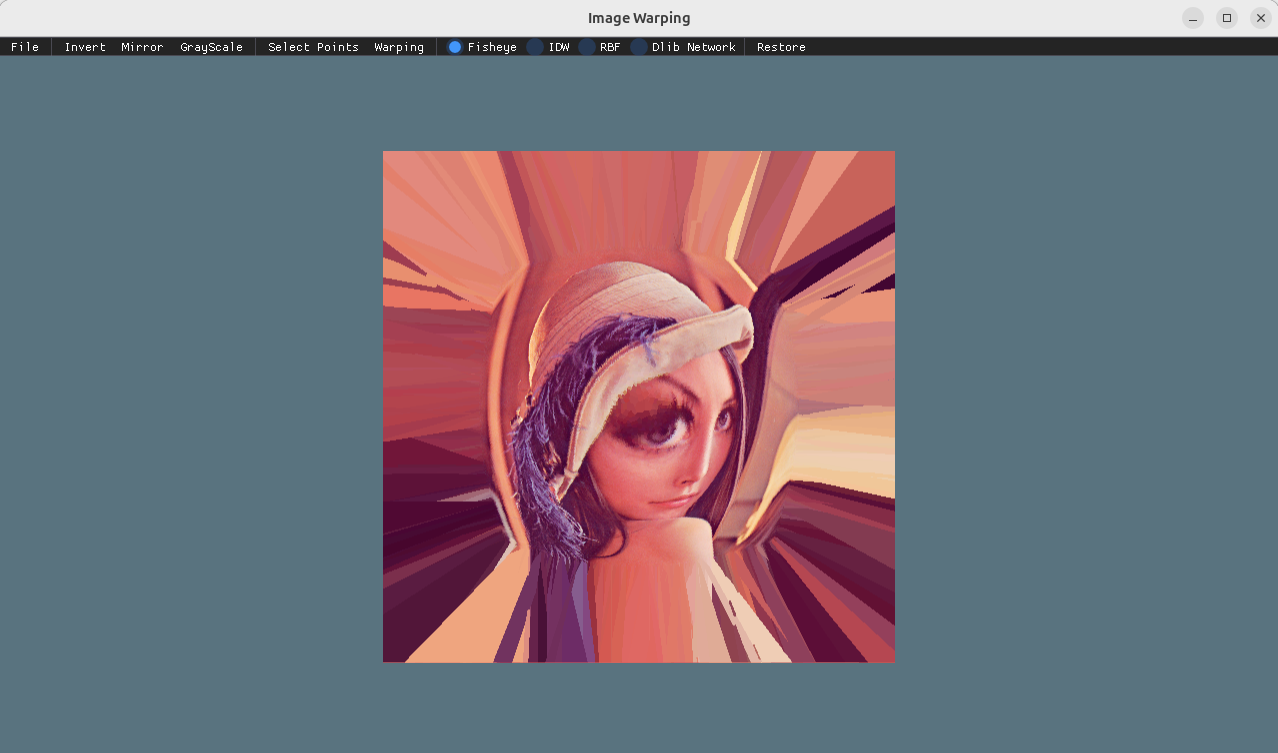
\includegraphics[width=\textwidth]{example_pictures/lenna_fisheye.png}
        \caption{Lenna 鱼眼与缝隙修复算法}
    \end{subfigure}
    \hfill
    \begin{subfigure}{0.45\textwidth}
        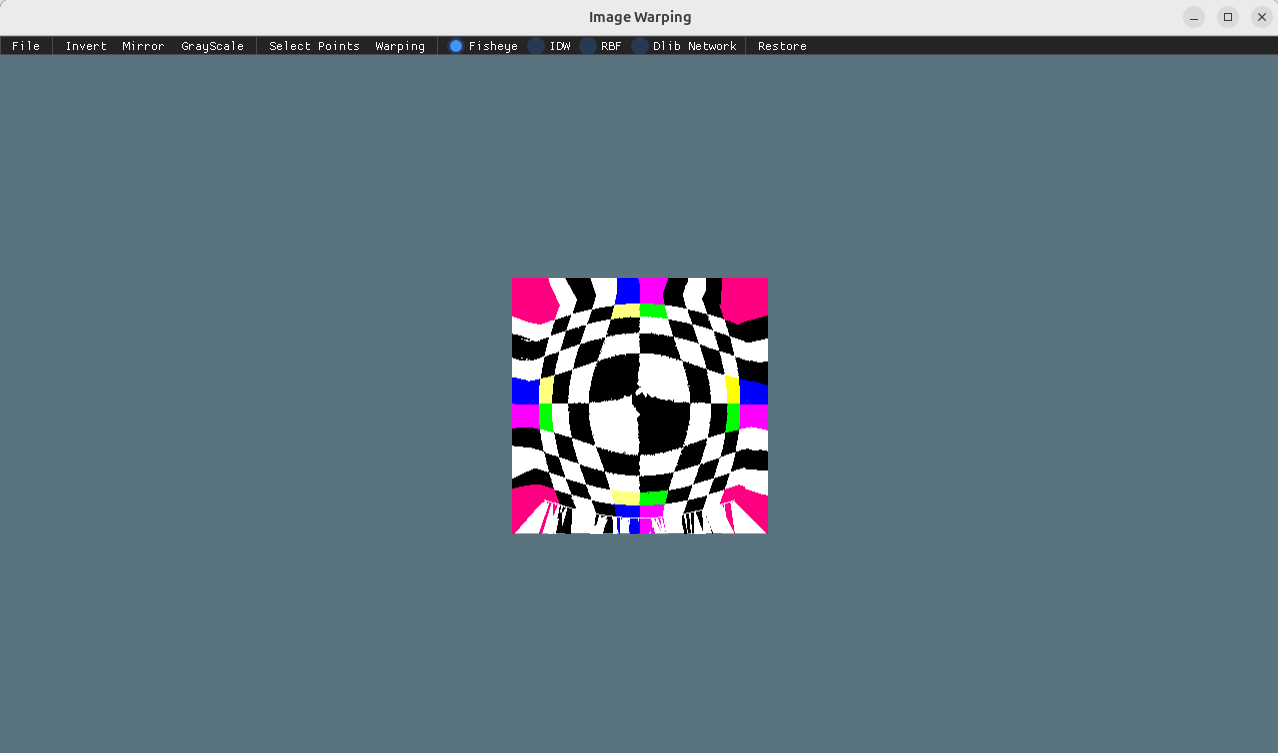
\includegraphics[width=\textwidth]{example_pictures/棋盘格_fisheye.png}
        \caption{棋盘格 鱼眼与缝隙修复算法}
    \end{subfigure}
    \caption{前向映射（鱼眼）与 ANN 像素孔填充渲染}
\end{figure}

\section{总结}
本次实验顺利实践了 C++ 的面向对象规范，掌握并自主实现了图像逆向与正向映射的系统级差异。通过对线性方程解库进行原生化高斯消除法重制、以及为前向过程应用 Spotify Annoy 树进行黑白缝修复，达成了出色的视觉观感。同时在 C++ 层接入 Dlib 库，实现了通过深度前馈网络回归训练直接映射点集，大幅拓宽和增强了作业的完整度和扩展挑战。

\end{document}
